% GNUPLOT: LaTeX picture with Postscript
\begingroup
  \makeatletter
  \providecommand\color[2][]{%
    \GenericError{(gnuplot) \space\space\space\@spaces}{%
      Package color not loaded in conjunction with
      terminal option `colourtext'%
    }{See the gnuplot documentation for explanation.%
    }{Either use 'blacktext' in gnuplot or load the package
      color.sty in LaTeX.}%
    \renewcommand\color[2][]{}%
  }%
  \providecommand\includegraphics[2][]{%
    \GenericError{(gnuplot) \space\space\space\@spaces}{%
      Package graphicx or graphics not loaded%
    }{See the gnuplot documentation for explanation.%
    }{The gnuplot epslatex terminal needs graphicx.sty or graphics.sty.}%
    \renewcommand\includegraphics[2][]{}%
  }%
  \providecommand\rotatebox[2]{#2}%
  \@ifundefined{ifGPcolor}{%
    \newif\ifGPcolor
    \GPcolorfalse
  }{}%
  \@ifundefined{ifGPblacktext}{%
    \newif\ifGPblacktext
    \GPblacktexttrue
  }{}%
  % define a \g@addto@macro without @ in the name:
  \let\gplgaddtomacro\g@addto@macro
  % define empty templates for all commands taking text:
  \gdef\gplbacktext{}%
  \gdef\gplfronttext{}%
  \makeatother
  \ifGPblacktext
    % no textcolor at all
    \def\colorrgb#1{}%
    \def\colorgray#1{}%
  \else
    % gray or color?
    \ifGPcolor
      \def\colorrgb#1{\color[rgb]{#1}}%
      \def\colorgray#1{\color[gray]{#1}}%
      \expandafter\def\csname LTw\endcsname{\color{white}}%
      \expandafter\def\csname LTb\endcsname{\color{black}}%
      \expandafter\def\csname LTa\endcsname{\color{black}}%
      \expandafter\def\csname LT0\endcsname{\color[rgb]{1,0,0}}%
      \expandafter\def\csname LT1\endcsname{\color[rgb]{0,1,0}}%
      \expandafter\def\csname LT2\endcsname{\color[rgb]{0,0,1}}%
      \expandafter\def\csname LT3\endcsname{\color[rgb]{1,0,1}}%
      \expandafter\def\csname LT4\endcsname{\color[rgb]{0,1,1}}%
      \expandafter\def\csname LT5\endcsname{\color[rgb]{1,1,0}}%
      \expandafter\def\csname LT6\endcsname{\color[rgb]{0,0,0}}%
      \expandafter\def\csname LT7\endcsname{\color[rgb]{1,0.3,0}}%
      \expandafter\def\csname LT8\endcsname{\color[rgb]{0.5,0.5,0.5}}%
    \else
      % gray
      \def\colorrgb#1{\color{black}}%
      \def\colorgray#1{\color[gray]{#1}}%
      \expandafter\def\csname LTw\endcsname{\color{white}}%
      \expandafter\def\csname LTb\endcsname{\color{black}}%
      \expandafter\def\csname LTa\endcsname{\color{black}}%
      \expandafter\def\csname LT0\endcsname{\color{black}}%
      \expandafter\def\csname LT1\endcsname{\color{black}}%
      \expandafter\def\csname LT2\endcsname{\color{black}}%
      \expandafter\def\csname LT3\endcsname{\color{black}}%
      \expandafter\def\csname LT4\endcsname{\color{black}}%
      \expandafter\def\csname LT5\endcsname{\color{black}}%
      \expandafter\def\csname LT6\endcsname{\color{black}}%
      \expandafter\def\csname LT7\endcsname{\color{black}}%
      \expandafter\def\csname LT8\endcsname{\color{black}}%
    \fi
  \fi
    \setlength{\unitlength}{0.0500bp}%
    \ifx\gptboxheight\undefined%
      \newlength{\gptboxheight}%
      \newlength{\gptboxwidth}%
      \newsavebox{\gptboxtext}%
    \fi%
    \setlength{\fboxrule}{0.5pt}%
    \setlength{\fboxsep}{1pt}%
    \definecolor{tbcol}{rgb}{1,1,1}%
\begin{picture}(6336.00,4030.00)%
    \gplgaddtomacro\gplbacktext{%
      \csname LTb\endcsname%%
      \put(5855,440){\makebox(0,0)[r]{\strut{}}}%
      \csname LTb\endcsname%%
      \put(5855,609){\makebox(0,0)[r]{\strut{}}}%
      \csname LTb\endcsname%%
      \put(5855,779){\makebox(0,0)[r]{\strut{}}}%
      \csname LTb\endcsname%%
      \put(5855,948){\makebox(0,0)[r]{\strut{}}}%
      \csname LTb\endcsname%%
      \put(5855,1118){\makebox(0,0)[r]{\strut{}}}%
      \csname LTb\endcsname%%
      \put(5855,1287){\makebox(0,0)[r]{\strut{}}}%
      \csname LTb\endcsname%%
      \put(5855,1457){\makebox(0,0)[r]{\strut{}}}%
      \csname LTb\endcsname%%
      \put(5855,1626){\makebox(0,0)[r]{\strut{}}}%
      \csname LTb\endcsname%%
      \put(5855,1796){\makebox(0,0)[r]{\strut{}}}%
      \csname LTb\endcsname%%
      \put(5855,1965){\makebox(0,0)[r]{\strut{}}}%
      \csname LTb\endcsname%%
      \put(5855,2135){\makebox(0,0)[r]{\strut{}}}%
      \csname LTb\endcsname%%
      \put(5855,2304){\makebox(0,0)[r]{\strut{}}}%
      \csname LTb\endcsname%%
      \put(5855,2473){\makebox(0,0)[r]{\strut{}}}%
      \csname LTb\endcsname%%
      \put(5855,2643){\makebox(0,0)[r]{\strut{}}}%
      \csname LTb\endcsname%%
      \put(5855,2812){\makebox(0,0)[r]{\strut{}}}%
      \csname LTb\endcsname%%
      \put(5855,2982){\makebox(0,0)[r]{\strut{}}}%
      \csname LTb\endcsname%%
      \put(5855,3151){\makebox(0,0)[r]{\strut{}}}%
      \csname LTb\endcsname%%
      \put(5855,3321){\makebox(0,0)[r]{\strut{}}}%
      \csname LTb\endcsname%%
      \put(5855,3490){\makebox(0,0)[r]{\strut{}}}%
      \csname LTb\endcsname%%
      \put(5855,3660){\makebox(0,0)[r]{\strut{}}}%
      \csname LTb\endcsname%%
      \put(5855,3829){\makebox(0,0)[r]{\strut{}}}%
      \csname LTb\endcsname%%
      \put(500,240){\makebox(0,0){\strut{}}}%
      \csname LTb\endcsname%%
      \put(956,240){\makebox(0,0){\strut{}}}%
      \csname LTb\endcsname%%
      \put(1412,240){\makebox(0,0){\strut{}}}%
      \csname LTb\endcsname%%
      \put(1869,240){\makebox(0,0){\strut{}}}%
      \csname LTb\endcsname%%
      \put(2325,240){\makebox(0,0){\strut{}}}%
      \csname LTb\endcsname%%
      \put(2781,240){\makebox(0,0){\strut{}}}%
      \csname LTb\endcsname%%
      \put(3237,240){\makebox(0,0){\strut{}}}%
      \csname LTb\endcsname%%
      \put(3694,240){\makebox(0,0){\strut{}}}%
      \csname LTb\endcsname%%
      \put(4150,240){\makebox(0,0){\strut{}}}%
      \csname LTb\endcsname%%
      \put(4606,240){\makebox(0,0){\strut{}}}%
      \csname LTb\endcsname%%
      \put(5062,240){\makebox(0,0){\strut{}}}%
      \csname LTb\endcsname%%
      \put(5519,240){\makebox(0,0){\strut{}}}%
      \csname LTb\endcsname%%
      \put(5975,240){\makebox(0,0){\strut{}}}%
      \csname LTb\endcsname%%
      \put(500,271){\makebox(0,0)[l]{\strut{}-1.135}}%
      \put(1184,271){\makebox(0,0)[l]{\strut{}-1.098}}%
      \put(1869,271){\makebox(0,0)[l]{\strut{}-1.037}}%
      \put(6112,3575){\makebox(0,0)[l]{\strut{}18.5}}%
      \put(6112,3405){\makebox(0,0)[l]{\strut{}17.7}}%
      \put(6112,3151){\makebox(0,0)[l]{\strut{}15.8}}%
    }%
    \gplgaddtomacro\gplfronttext{%
      \csname LTb\endcsname%%
      \put(190,2134){\rotatebox{-270.00}{\makebox(0,0){\strut{}$I_{\text{D}}[mA]$}}}%
      \put(3237,140){\makebox(0,0){\strut{}$V_{\text{GS}}[V]$}}%
    }%
    \gplgaddtomacro\gplbacktext{%
      \csname LTb\endcsname%%
      \put(5855,440){\makebox(0,0)[r]{\strut{}}}%
      \csname LTb\endcsname%%
      \put(5855,609){\makebox(0,0)[r]{\strut{}}}%
      \csname LTb\endcsname%%
      \put(5855,779){\makebox(0,0)[r]{\strut{}}}%
      \csname LTb\endcsname%%
      \put(5855,948){\makebox(0,0)[r]{\strut{}}}%
      \csname LTb\endcsname%%
      \put(5855,1118){\makebox(0,0)[r]{\strut{}}}%
      \csname LTb\endcsname%%
      \put(5855,1287){\makebox(0,0)[r]{\strut{}}}%
      \csname LTb\endcsname%%
      \put(5855,1457){\makebox(0,0)[r]{\strut{}}}%
      \csname LTb\endcsname%%
      \put(5855,1626){\makebox(0,0)[r]{\strut{}}}%
      \csname LTb\endcsname%%
      \put(5855,1796){\makebox(0,0)[r]{\strut{}}}%
      \csname LTb\endcsname%%
      \put(5855,1965){\makebox(0,0)[r]{\strut{}}}%
      \csname LTb\endcsname%%
      \put(5855,2135){\makebox(0,0)[r]{\strut{}}}%
      \csname LTb\endcsname%%
      \put(5855,2304){\makebox(0,0)[r]{\strut{}}}%
      \csname LTb\endcsname%%
      \put(5855,2473){\makebox(0,0)[r]{\strut{}}}%
      \csname LTb\endcsname%%
      \put(5855,2643){\makebox(0,0)[r]{\strut{}}}%
      \csname LTb\endcsname%%
      \put(5855,2812){\makebox(0,0)[r]{\strut{}}}%
      \csname LTb\endcsname%%
      \put(5855,2982){\makebox(0,0)[r]{\strut{}}}%
      \csname LTb\endcsname%%
      \put(5855,3151){\makebox(0,0)[r]{\strut{}}}%
      \csname LTb\endcsname%%
      \put(5855,3321){\makebox(0,0)[r]{\strut{}}}%
      \csname LTb\endcsname%%
      \put(5855,3490){\makebox(0,0)[r]{\strut{}}}%
      \csname LTb\endcsname%%
      \put(5855,3660){\makebox(0,0)[r]{\strut{}}}%
      \csname LTb\endcsname%%
      \put(5855,3829){\makebox(0,0)[r]{\strut{}}}%
      \csname LTb\endcsname%%
      \put(500,240){\makebox(0,0){\strut{}}}%
      \csname LTb\endcsname%%
      \put(956,240){\makebox(0,0){\strut{}}}%
      \csname LTb\endcsname%%
      \put(1412,240){\makebox(0,0){\strut{}}}%
      \csname LTb\endcsname%%
      \put(1869,240){\makebox(0,0){\strut{}}}%
      \csname LTb\endcsname%%
      \put(2325,240){\makebox(0,0){\strut{}}}%
      \csname LTb\endcsname%%
      \put(2781,240){\makebox(0,0){\strut{}}}%
      \csname LTb\endcsname%%
      \put(3237,240){\makebox(0,0){\strut{}}}%
      \csname LTb\endcsname%%
      \put(3694,240){\makebox(0,0){\strut{}}}%
      \csname LTb\endcsname%%
      \put(4150,240){\makebox(0,0){\strut{}}}%
      \csname LTb\endcsname%%
      \put(4606,240){\makebox(0,0){\strut{}}}%
      \csname LTb\endcsname%%
      \put(5062,240){\makebox(0,0){\strut{}}}%
      \csname LTb\endcsname%%
      \put(5519,240){\makebox(0,0){\strut{}}}%
      \csname LTb\endcsname%%
      \put(5975,240){\makebox(0,0){\strut{}}}%
      \csname LTb\endcsname%%
      \put(500,271){\makebox(0,0)[l]{\strut{}-1.135}}%
      \put(1184,271){\makebox(0,0)[l]{\strut{}-1.098}}%
      \put(1869,271){\makebox(0,0)[l]{\strut{}-1.037}}%
      \put(6112,3575){\makebox(0,0)[l]{\strut{}18.5}}%
      \put(6112,3405){\makebox(0,0)[l]{\strut{}17.7}}%
      \put(6112,3151){\makebox(0,0)[l]{\strut{}15.8}}%
    }%
    \gplgaddtomacro\gplfronttext{%
      \csname LTb\endcsname%%
      \put(190,2134){\rotatebox{-270.00}{\makebox(0,0){\strut{}$I_{\text{D}}[mA]$}}}%
      \put(3237,140){\makebox(0,0){\strut{}$V_{\text{GS}}[V]$}}%
    }%
    \gplgaddtomacro\gplbacktext{%
      \csname LTb\endcsname%%
      \put(5855,440){\makebox(0,0)[r]{\strut{}}}%
      \csname LTb\endcsname%%
      \put(5855,609){\makebox(0,0)[r]{\strut{}}}%
      \csname LTb\endcsname%%
      \put(5855,779){\makebox(0,0)[r]{\strut{}}}%
      \csname LTb\endcsname%%
      \put(5855,948){\makebox(0,0)[r]{\strut{}}}%
      \csname LTb\endcsname%%
      \put(5855,1118){\makebox(0,0)[r]{\strut{}}}%
      \csname LTb\endcsname%%
      \put(5855,1287){\makebox(0,0)[r]{\strut{}}}%
      \csname LTb\endcsname%%
      \put(5855,1457){\makebox(0,0)[r]{\strut{}}}%
      \csname LTb\endcsname%%
      \put(5855,1626){\makebox(0,0)[r]{\strut{}}}%
      \csname LTb\endcsname%%
      \put(5855,1796){\makebox(0,0)[r]{\strut{}}}%
      \csname LTb\endcsname%%
      \put(5855,1965){\makebox(0,0)[r]{\strut{}}}%
      \csname LTb\endcsname%%
      \put(5855,2135){\makebox(0,0)[r]{\strut{}}}%
      \csname LTb\endcsname%%
      \put(5855,2304){\makebox(0,0)[r]{\strut{}}}%
      \csname LTb\endcsname%%
      \put(5855,2473){\makebox(0,0)[r]{\strut{}}}%
      \csname LTb\endcsname%%
      \put(5855,2643){\makebox(0,0)[r]{\strut{}}}%
      \csname LTb\endcsname%%
      \put(5855,2812){\makebox(0,0)[r]{\strut{}}}%
      \csname LTb\endcsname%%
      \put(5855,2982){\makebox(0,0)[r]{\strut{}}}%
      \csname LTb\endcsname%%
      \put(5855,3151){\makebox(0,0)[r]{\strut{}}}%
      \csname LTb\endcsname%%
      \put(5855,3321){\makebox(0,0)[r]{\strut{}}}%
      \csname LTb\endcsname%%
      \put(5855,3490){\makebox(0,0)[r]{\strut{}}}%
      \csname LTb\endcsname%%
      \put(5855,3660){\makebox(0,0)[r]{\strut{}}}%
      \csname LTb\endcsname%%
      \put(5855,3829){\makebox(0,0)[r]{\strut{}}}%
      \csname LTb\endcsname%%
      \put(500,240){\makebox(0,0){\strut{}}}%
      \csname LTb\endcsname%%
      \put(956,240){\makebox(0,0){\strut{}}}%
      \csname LTb\endcsname%%
      \put(1412,240){\makebox(0,0){\strut{}}}%
      \csname LTb\endcsname%%
      \put(1869,240){\makebox(0,0){\strut{}}}%
      \csname LTb\endcsname%%
      \put(2325,240){\makebox(0,0){\strut{}}}%
      \csname LTb\endcsname%%
      \put(2781,240){\makebox(0,0){\strut{}}}%
      \csname LTb\endcsname%%
      \put(3237,240){\makebox(0,0){\strut{}}}%
      \csname LTb\endcsname%%
      \put(3694,240){\makebox(0,0){\strut{}}}%
      \csname LTb\endcsname%%
      \put(4150,240){\makebox(0,0){\strut{}}}%
      \csname LTb\endcsname%%
      \put(4606,240){\makebox(0,0){\strut{}}}%
      \csname LTb\endcsname%%
      \put(5062,240){\makebox(0,0){\strut{}}}%
      \csname LTb\endcsname%%
      \put(5519,240){\makebox(0,0){\strut{}}}%
      \csname LTb\endcsname%%
      \put(5975,240){\makebox(0,0){\strut{}}}%
      \csname LTb\endcsname%%
      \put(500,271){\makebox(0,0)[l]{\strut{}-1.135}}%
      \put(1184,271){\makebox(0,0)[l]{\strut{}-1.098}}%
      \put(1869,271){\makebox(0,0)[l]{\strut{}-1.037}}%
      \put(6112,3575){\makebox(0,0)[l]{\strut{}18.5}}%
      \put(6112,3405){\makebox(0,0)[l]{\strut{}17.7}}%
      \put(6112,3151){\makebox(0,0)[l]{\strut{}15.8}}%
    }%
    \gplgaddtomacro\gplfronttext{%
      \csname LTb\endcsname%%
      \put(190,2134){\rotatebox{-270.00}{\makebox(0,0){\strut{}$I_{\text{D}}[mA]$}}}%
      \put(3237,140){\makebox(0,0){\strut{}$V_{\text{GS}}[V]$}}%
    }%
    \gplbacktext
    \put(0,0){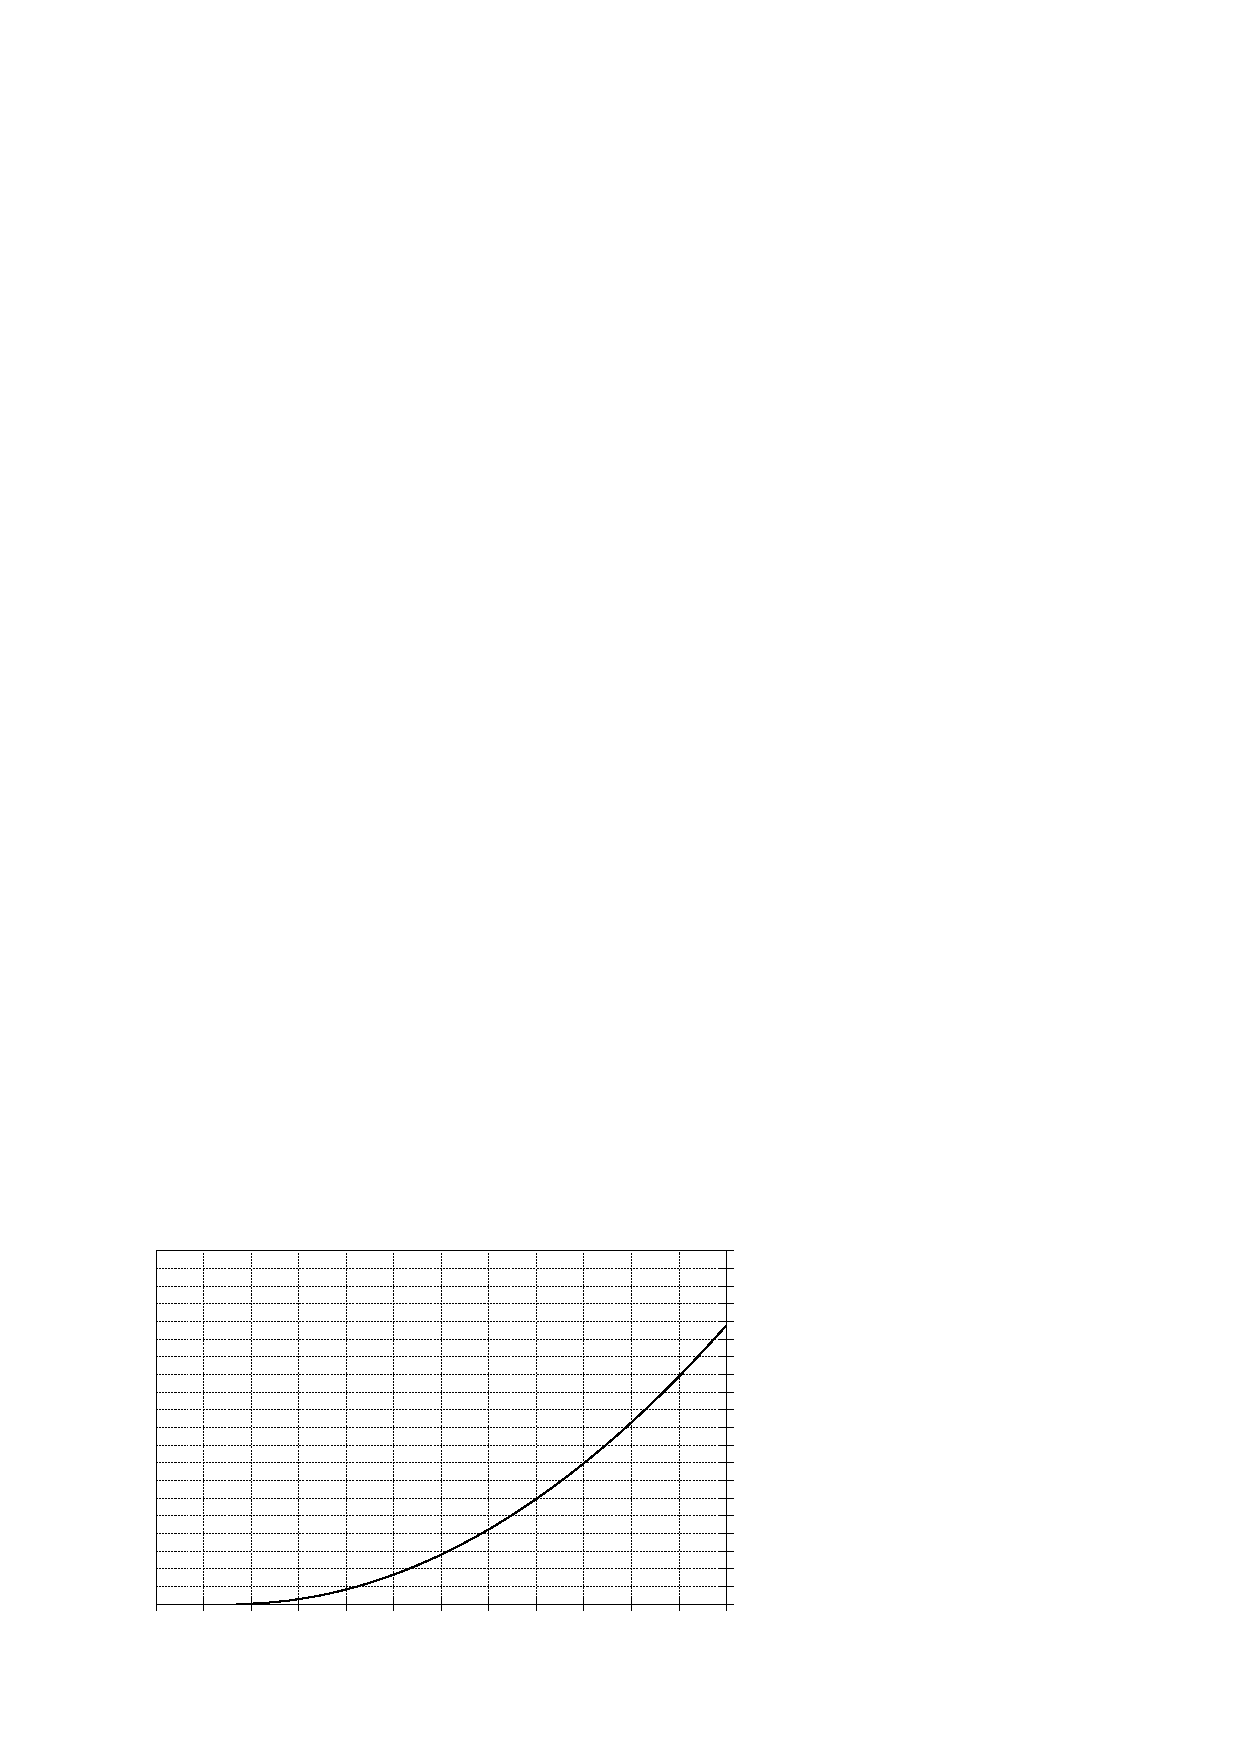
\includegraphics[width={316.80bp},height={201.50bp}]{curva1}}%
    \gplfronttext
  \end{picture}%
\endgroup
